\section{实验}
\label{sec:experiments}

\subsection{实验设计}

\textbf{数据集。} 本实验选取了两个具有代表性的数学问题数据集:GSM8K\citep{cobbe2021training}和MATH\citep{hendrycksmath2021}。GSM8K数据集由OpenAI发布,包含8.5K个小学数学问题,这些问题覆盖了基础的算术运算,适合用来评估模型对基础数学问题的处理能力。MATH数据集则由加州大学伯克利分校的研究团队开发,包含12,500个来自高中数学的问题,这些问题的难度更高,覆盖了更广泛的数学领域,适合用来评估模型对较复杂数学问题的推理能力。在本实验中,测试集分别为GSM8K的test子集,以及MATH500子集,以便于对比和分析。

\textbf{模型。} 实验中主要使用了Qwen2.5系列模型\citep{qwen2.5},这是一个基于LLM(Large Language Models)的模型家族,提供了不同规模的模型以适应不同的计算资源和任务需求。具体来说,我们使用了0.5B和1.5B两种规模的模型进行实验。这些模型均在Hugging Face平台上提供,便于进行微调和部署。

\textbf{实验环境配置。} 
为了确保实验结果的可靠性并且提高实验的效率,本研究在最终实验阶段租用了AutoDL平台的服务器,使用了如下配置的计算平台进行实验:
\begin{itemize}
    \item \textbf{硬件配置}:
        \begin{itemize}
            \item \textbf{图形处理单元 (GPU)}: NVIDIA GeForce RTX 4090, 24GB GDDR6X 
            \item \textbf{中央处理器 (CPU)}: Intel (R) Xeon (R) Platinum 8481C,16 CPU
            \item \textbf{内存}: 80GB RAM
        \end{itemize}
    \item \textbf{软件配置}:
        \begin{itemize}
            \item \textbf{操作系统}: Ubuntu 22.04 LTS
            \item \textbf{编程语言}: Python 3.12
            \item \textbf{深度学习框架}: PyTorch 2.5.1
            \item \textbf{CUDA 版本}: CUDA Toolkit 12.4 \end{itemize}
\end{itemize}

\subsection{实验结果} 

\begin{figure}[htbp]
    \centering
    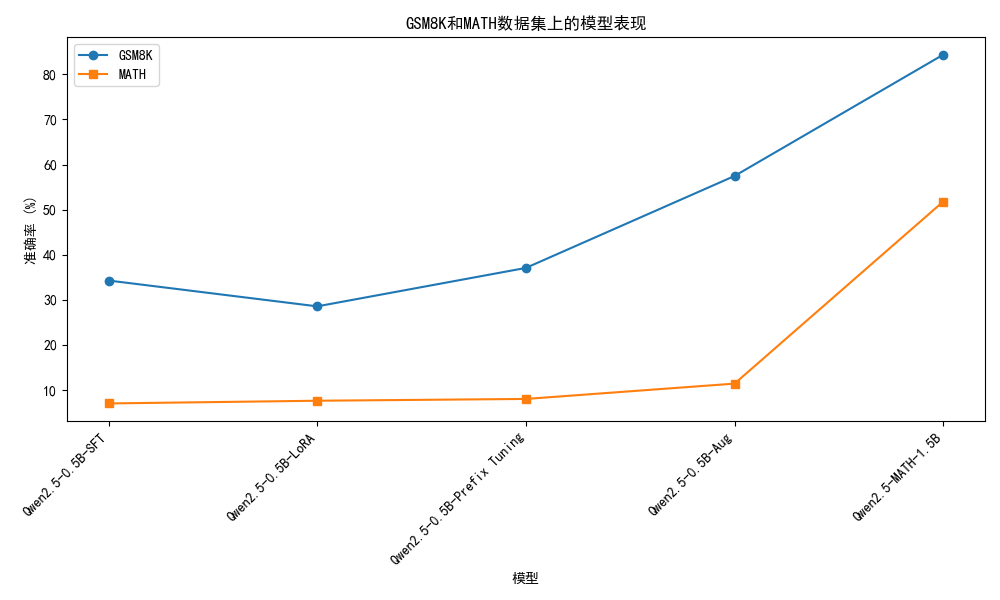
\includegraphics[width=0.9\textwidth]{figs/model_acc.png} 
    \caption{不同方法在GSM8K和MATH数据集上的准确率对比}
    \label{fig:experiment_result}
\end{figure}

\textbf{主要结果。} 
 表格\ref{fig:experiment_result}总结了各个模型在 GSM8K 和 MATH 数据集上的准确率。结果显示,在 GSM8K 数据集上,Qwen2.5-0.5B-SFT、Qwen2.5-0.5B-LoRA、Qwen2.5-0.5B-Prefix Tuning、Qwen2.5-0.5B-Aug 和 Qwen2.5-MATH-1.5B的生成结果分别达到了34.27\%、28.54\%、37.07\%、57.47\%和84.38\%的准确率;而在 MATH 数据集上,分别达到了7.00\%、7.60\%、8.00\%、11.40\%和51.80\%的准确率。

\textbf{不同方法的影响}
\begin{itemize}
    \item \textbf{监督微调(SFT)}:作为基线模型,SFT 展示了模型在简单训练的情况下处理数学问题的能力,参数量仅仅0.5B的模型在SFT后即可完成一部分简单数学题目,在GSM8K和MATH数据集上准确率分别为34.27\%和7.00\%,在实验环境中训练用时合计约60分钟。
    \item \textbf{LoRA 技术}:通过使用 LoRA 进行微调,我们观察到相比于 SFT,在在 GSM8K 数据集上准确率下降了 5.73\%,而在 MATH 数据集上准确率提高了 0.6\%。这可能是由于 LoRA 的参数高效特性限制了模型学习新知识的能力,特别是在面对求解数学题这一复杂任务时。然而,LoRA 的优势在于显著减少了计算资源的需求,使得大规模模型的微调成为可能,在实验环境中训练用时合计约20分钟。
    \item \textbf{Prefix Tuning技术}:Prefix Tuning展示了其卓越的适应能力。由于Prefix Tuning只引入了额外的前缀向量,不会改变原始模型参数,可以缓解传统微调过程中的灾难性遗忘问题,提高性能。实验结果显示,Prefix Tuning不仅在资源受限条件下缩短了训练时间和显存占用,在GSM8K和MATH数据集上,Prefix Tuning的表现均优于完全微调的基线模型,分别提升了23.20\%和4.40\%。在实验环境中,Prefix Tuning的训练用时合计约40分钟。
    \item \textbf{查询响应增强}:查询响应增强技术通过引入更复杂和多样化的问题表述以及多个推理路径,显著提升了数据集的质量和多样性。这种方法促进了模型对问题更深层次的理解。实验结果表明,应用查询响应增强后的模型在复杂数学推理任务上表现略有提升,在GSM8K和MATH数据集上的准确率分别提升了2.80\%和1.00\%,但是数据量较大,在实验环境中训练用时合计约180分钟。
    \item \textbf{MATH专家模型}:针对资源受限的情况,我们选择了专门为数学领域优化的大模型Qwen2.5-MATH-1.5B进行测试。实验显示,该模型在增加了参数量,而且在专业数学数据集上进行了预训练的情况下,在数学推理任务上展现了极高的准确率,在GSM8K和MATH数据集上的准确率分别提升了50.11\%和44.80\%,达到了84.38\%和51.80\%。该模型未在本地进行训练。
\end{itemize}

\subsection{结果分析} 
\subsubsection{高效微调与数据增强的性能影响分析}

高效微调技术在资源受限条件下的应用展现了显著的优势。LoRA在计算资源消耗上性能优越,然而其在GSM8K数据集上性能下降的现象揭示了这样一种可能:在任务的复杂性和需要捕捉的知识结构较为动态的场景中,LoRA的表达能力可能受限。这限制了其在复杂推理任务中的适应性和灵活性。

相比之下,Prefix Tuning技术展示了其优越的适应能力。这种方法有效地缓解了灾难性遗忘问题,在不增加计算复杂度的同时,提升了模型在新任务上的性能表现。在GSM8K和MATH数据集上的卓越表现说明,Prefix Tuning不仅保留了基础模型的知识架构,还为模型理解和应对高度复杂的推理任务提供了强有力的支持。

在数据增强方面,查询响应增强策略通过复杂化输入问题和多样化推理路径,提升了模型训练数据集的多样性和质量。这一方法增强了模型在复杂数学推理任务中的理解深度和泛化性能,但也增加了学习负担,训练时间翻倍。实验结果显示,尽管准确率略有提升,但在小模型参数规模下,数据增强对模型推理能力的提升有限,因模型对数据的理解能力本身受限。

\subsubsection{GSM8K vs. MATH 性能差异} 
从整体上看,模型在 GSM8K 上的表现明显优于 MATH 数据集。这一现象可以归因于两个数据集的性质差异:GSM8K 主要包含小学级别的基础算术运算问题,而 MATH 则涵盖了高中水平的复杂数学概念和推理问题。因此,MATH 数据集对模型提出了更高的要求,不仅需要理解复杂的数学符号和术语,还需要进行多步逻辑推理。这种复杂性增加了模型出错的概率,从而导致了较低的准确率。值得注意的是,MATH 数据集在 MATH 专家模型方法下的提升幅度明显高于 GSM8K 数据集,可能是因为该方法的大模型 Qwen2.5-MATH-1.5B 专为数学领域优化并在专业数学数据集上预训练,能够更有效地处理复杂的数学概念和推理任务。这种专门的优化使得模型对 MATH 数据集的复杂性具有更强的适应能力,从而显著提升准确率。
